

\section{From Shared-Memory to Distributed-\\Memory Environments}

In the previous sections, we have introduced our implementations on top of BaseX
and the evaluation with a single BaseX server on a dual-CPU system. As
introduced in the original study, data partitioning strategy was studied in a
shared-memory environment, where XML data is stored in a shared memory and can
be concurrently accessible by multiple XPath processors. In the conclusion of
the original paper~\cite{BoLS09},  the authors had pointed out that the
parallelization model is over XML data model, and it can also be adapted to any
XML storage laryout. However,  no matter in the original study, or in our
previous study, the strategies  are applied both in a shared-memory environment. 

Based on our previous experiment results, it would also be promising to use
multiple BaseX servers on multiple CPUs in distributed-memory environments over
large XML documents so that we can exploiting computer clusters to process 
them more efficiently. Then, here comes a question:  how we can apply it in a
distributed-memory environment over a number of computers? 
In this study, by exploiting horizontal fragmentation on XML data, we present our
study on applying data partitioning in a distributed-memory  environment to
experimentally show how it improves the scalability.



\section{Fragmentation}

\subsection{Introduction}
Fragmentation is an effective way to improve scalability of database
systems~\cite{navathe1995mixed, hauglid2010dyfram, khan2010new}.  In the field
of parallel XML processing, there are also some studies on  fragmentation of XML
data~\cite{kling11:dist_xml, KlOD10}.  The most common XML fragmentations are
horizontal fragmentation and vertical fragmentation~\cite{kling11:dist_xml}. Due
to the nature of horizontal fragments that are  relatively independent, it is a
more direct and practical way to work together with data partitioning. We thus
focus on only horizontal fragmentation in this study.

\subsection{Definitions}

To process a large XML document in a distrubed-memory environment, 
we first need to fragment the XML into multiple fragment that will
be allocated to computing node for querying. To make the fragments
well balanced, we introduce a fragmentation algorithm. We introduce 
the algorithm with an example in this section.

\subsubsection{Fragment}
We first define horizontal fragmentation. In this study, a \emph{fragment} 
is a collection of subtrees.
Since the mainpurpose of fragmentation is to achieve good scalability, we
attempt to make our fragmentation algorithm size-balanced, i.e. to make each
fragment have nearly the same amount of node. 
Therefore, a fragment satisfies two condictions. Firstly,
the roots of subtrees in a fragment are consecutive children of a single 
node in the input tree. Secondly, the number of elements in a fragment is 
less than or equal to a given integer \emph{maxsize}. 
Let us take the tree in Fig.~\ref{fig:frag_wholetree} as an example. Let 
maxsize be 5, then we have the fragments shown in Figure~\ref{fig:frag_fragmentation}.
After applying horizontal fragmentation to the example XML tree,
we obtain eight fragments enclosed in dotted rectangles.

%Let $D$ = \{$d_1$, $d_2$, ..., $d_n$\} be a collection of document trees such
%that each $d_i \in D$ conforms the same XML schema~\cite{xmlschema}.   Let
%$\mathit{FS}$ = \{$F_1$, $F_2$,..., $F_m$\}  be a collection of fragments such
%that for each $F_i \subset D$. If $\bigcup\limits_{i=1}^{m} F_{i} = F$ and
%$\bigcap\limits_{i=1}^{m} F_{i} = \emptyset$, then $\mathit{FS}$ is a
%\emph{horizontal fragmentation} of $D$.

\begin{figure}[t] 
	\centering
	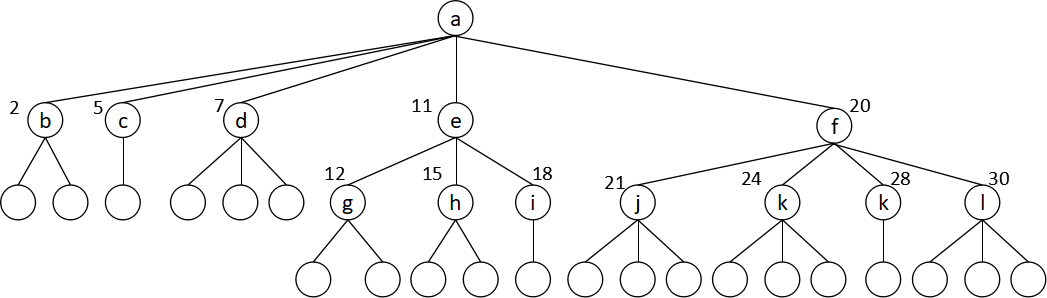
\includegraphics[scale=0.5]{frag_wholetree}
	\caption{An example tree and the PRE values along with nodes}
	\label{fig:frag_wholetree}
	
	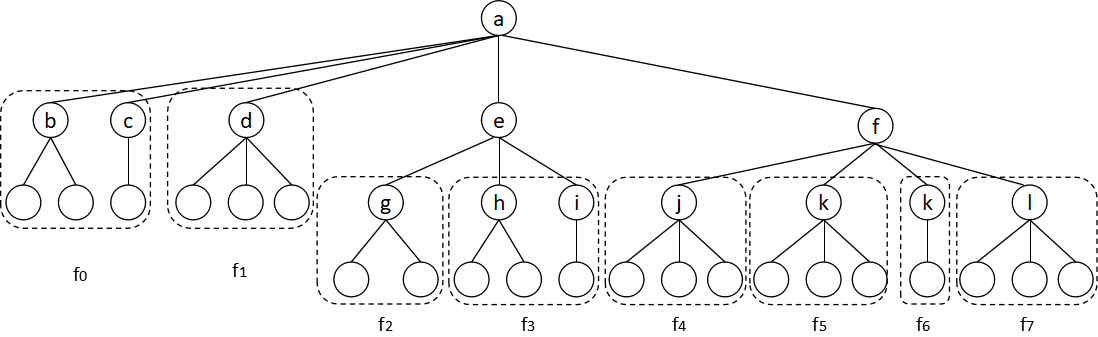
\includegraphics[scale=0.45]{frag_fragmentation}
	\caption{Fragmentation based on maxsize = 5.}
	\label{fig:frag_fragmentation}	
\end{figure}



\subsubsection{Anchored Fragment}

In order to ease performing top-down XPath queries, we augment
each fragment with the path from the root of the whole tree to the
subtrees.  We call this augmented fragment  \emph{anchored
fragment}. In the running example, we have eight anchored fragments as shown in Figure~\ref{fig:frag_anchortrees}.
 

\subsubsection{Root-merged Tree}

In most existing XML database management systems, such as BaseX, takes a 
single XML tree to create an XML database instance. Since a large number of 
databases instance arises overheads, we reduce the number of database 
instances by merging some of anchored fragments to \emph{root-merged tree}.
A root-merged tree is a number of anchored fragments merged at the root.
Note that we merge the root node of anchored fragments only, which is
enough to make list of fragments into a tree. 
For the running example, we can construct four root-merged trees from eight
fragments as shown in Figure~\ref{fig:frag_mergedtrees}.


\begin{figure}[t]   
	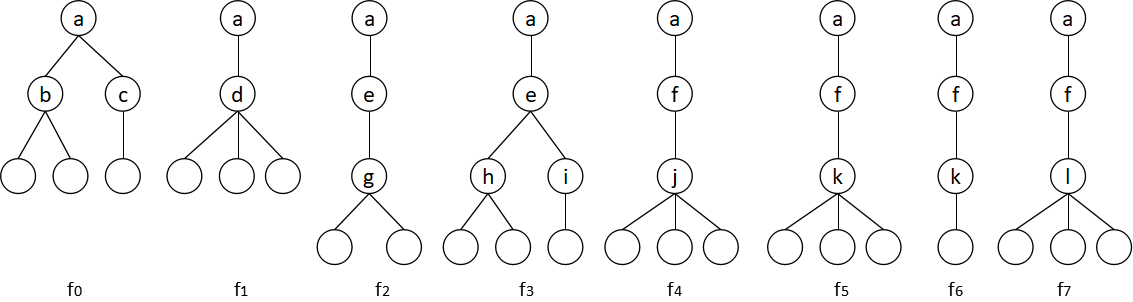
\includegraphics[scale=0.45]{frag_anchortrees}
	\caption{Anchor trees.}
	\label{fig:frag_anchortrees}	
	
	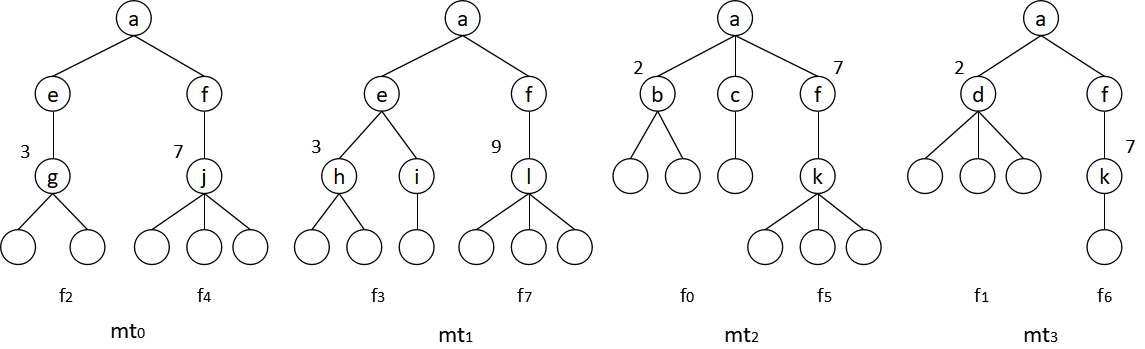
\includegraphics[scale=0.5]{frag_mergedtrees}
	\caption{Root-merged trees.}
	\label{fig:frag_mergedtrees}
\end{figure}

\subsubsection{Pruned Tree}
 
We can perform any XPath queries inside of a fragment, but we need
careful computation for XPath queries that may go out of the fragment.
In order to perform those XPath queries, we need to know the global
tree structure in which fragments are located.

For this purpose, we construct a "pruned tree" by replacing the subtrees
with a single node for each fragment.

In our running example, we have a pruned tree as shown in Figure~\ref{fig:frag_prunedtree}. 

In order to compute the pre-index in the input tree easily, we add
"gpre" for each node.  For the nodes representing pruned parts,
we add "fid" to link to the fragmentation index.

\begin{figure}[t]  
	\centering
	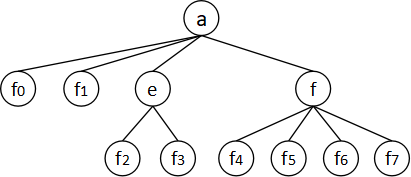
\includegraphics[scale=0.45]{frag_prunedtree}
	\caption{Pruned tree.}
	\label{fig:frag_prunedtree}	
\end{figure}


\subsection{Fragment Index}

The "fragment index" is the information required or useful for managing
fragments.  It has the following items for each fragment.
- fid: fragment ID
- mid: the root-merged tree that has the fragment
- mrank: the rank (position) of the fragment in the root-merged tree
- size: the size of fragments
- gpre: pre-index (in the input tree) of the first element
- mpre: pre-index (in the root-merged tree) of the first element

\begin{table}[t]
	
	\begin{tabular}{c|c|c|c|c|c}
			\caption{Fragment index.}
		\label{tab:fragmentindex}	
		\centering
		\hline
		 fid & mid    & mrank & size & gpre & mpre \\
		 \hline
		0   & mt0 & 0     &   5  & 2    & 2    \\
		1   & mt1 & 0     &   4  & 7    & 2    \\
		2   & mt2 & 0     &   3  & 12   & 3    \\
		3   & mt3 & 0     &   5  & 15   & 3    \\
		4   & mt4 & 1     &   4  & 18   & 4    \\
		5   & mt5 & 1     &   4  & 21   & 7    \\
		6   & mt6 & 1     &   2  & 24   & 7    \\
		7   & mt7 & 1     &   4  & 30   & 9    \\
		\hline
	\end{tabular}
\end{table}




\subsection{Fragmentation Algorithm}

We assume that all the results lie in the subtrees on the fragment. Thus,
to guarantee the correctness of query results, we need to guarantee the
completeness and uniqueness of nodes such that each node in the input XML tree
is included in at least a fragment. If a node is included a subtree part of a
fragment, then it is not included in any other fragment. 




\begin{figure}[]
	\centering
	\begin{tabular}{l}
		\hline
		\hline
		\makebox[.95\linewidth][l]{\textbf{Algorithm 1} \textsc{Fragmentation}($\mathit{nodes}$, $\mathit{MAXSIZE}$)} \\
		\hline
		\textbf{Input}:           $\mathit{nodes}$: a list of nodes, \\
		\makebox[1em][r]{}\hspace{9 mm}  $\mathit{MAXSIZE} $ : the maximum number of nodes in a fragment \\
		\textbf{Output}: a list of fragments \\
		\makebox[1em][r]{1:}\hspace{1 mm}  $\mathit{fragments} \leftarrow [] $     //a list of fragments \\
		\makebox[1em][r]{2:}\hspace{1 mm}  $subtrees \leftarrow [] $     //a list of root nodes of subtrees \\
		\makebox[1em][r]{3:}\hspace{1 mm}  \textbf{for all} $\emph{node} \in \emph{nodes}$ \textbf{do} \\
		\makebox[1em][r]{4:}\hspace{5 mm}  \textbf{if} \texttt{size($node$)} $ > \mathit{MAXSIZE} $ \textbf{then} \\
		\makebox[1em][r]{5:}\hspace{9 mm}  \textbf{if} $subtrees.length > 0$  \textbf{then} \\
		\makebox[1em][r]{6:}\hspace{13 mm} $\mathit{fragments}.Add((\textit{\_, subtrees}))$ \\
		\makebox[1em][r]{7:}\hspace{13 mm}  $\mathit{subtrees} \leftarrow []$ \\
		\makebox[1em][r]{8:}\hspace{9 mm}  \textbf{end if}\\
		\makebox[1em][r]{9:}\hspace{9 mm}  $\mathit{fragments}.AddAll($\texttt{Fragmentation}$($\texttt{child}$(node), \mathit{MAXSIZE}))$ \\
		\makebox[1em][r]{10:}\hspace{5 mm}  \textbf{else if} \texttt{size($node$)} + \texttt{Size}$(subtrees) > \mathit{MAXSIZE}$ \textbf{then} \\
		\makebox[1em][r]{11:}\hspace{9 mm} $\mathit{fragments}.Add((\_, subtrees))$ \\
		\makebox[1em][r]{12:}\hspace{9 mm} $subtrees \leftarrow [node]$ \\
		\makebox[1em][r]{13:}\hspace{5 mm}  \textbf{else}\\
		\makebox[1em][r]{14:}\hspace{9 mm} $\mathit{subtrees}.Add(node)$ \\
		\makebox[1em][r]{15:}\hspace{5 mm}  \textbf{end if}\\
		\makebox[1em][r]{16:}\hspace{1 mm}  \textbf{end for}\\
		\makebox[1em][r]{17:}\hspace{1 mm}  \textbf{for} $i \in [0, \mathit{fragments}.length)$ \textbf{do}\\
		\makebox[1em][r]{18:}\hspace{5 mm}  $\mathit{fragments}[i] \leftarrow $\texttt{AddPath}($\mathit{fragments}[i]$)  \\
		\makebox[1em][r]{19:}\hspace{1 mm}  \textbf{end for}\\
		\makebox[1em][r]{20:}\hspace{1 mm}  \textbf{return} $\mathit{fragments}$\\
		\hline
	\end{tabular}
	\caption{The fragmentation algorithm.}
	\label{fig:algQuery1}
\end{figure}


\begin{figure}[]
	\centering
	\begin{tabular}{l}
		\hline
		\hline
		\makebox[.95\linewidth][l]{\textbf{Algorithm 2} \textsc{AddPath}($\mathit{subtrees}$)} \\
		\hline
		\textbf{Input}:   $\mathit{subtrees}$: a list of root nodes of subtrees \\
		\textbf{Output}:  the root node of a tree that is augmented with the \\
		\makebox[1em][r]{}\hspace{13 mm}  path to the root of the whole tree\\
		\makebox[1em][r]{1:}\hspace{1 mm}  $\mathit{p} \leftarrow $\texttt{parent}$(subtrees[0]) $   \\
		\makebox[1em][r]{2:}\hspace{1 mm}  $node \leftarrow $ \texttt{clone}($p$)    \\
		\makebox[1em][r]{3:}\hspace{1 mm}  $node.addChildren(subtrees) $ \\
		\makebox[1em][r]{4:}\hspace{1 mm}  \textbf{while} \texttt{parent}$(p) \neq \mathit{NULL}$ \textbf{do}\\
		\makebox[1em][r]{5:}\hspace{5 mm}  $p \leftarrow $ \texttt{parent}($p$) \\
		\makebox[1em][r]{6:}\hspace{5 mm}  $tempnode \leftarrow$ \texttt{clone}($p$)  \\
		\makebox[1em][r]{7:}\hspace{5 mm}  $tempnode.addChild(node)$ \\
		\makebox[1em][r]{8:}\hspace{5 mm}  $node \leftarrow tempnode$ \\
		\makebox[1em][r]{9:}\hspace{1 mm}  \textbf{end while} \\
		\makebox[1em][r]{10:}\hspace{1 mm}  \textbf{return} $\mathit{node}$\\
		\hline
	\end{tabular}
	\caption{Add path to a list of subtrees}
	\label{fig:algQuery2}
\end{figure}





Algorithm 1 describes how our fragmentation works to apply a horizontal
fragmentation to a tree. The arguments of input are a list of nodes denoting the
tree to be fragmented and an integer number denoting the maximum number of nodes
a fragment can have so that we can make the fragments in similar size.   In Line
1--2, we declare an empty list of fragments and an empty list of subtrees for
holding results. In Line 3--16, we traverse each node in the input list, if the
node have more number of descendant nodes greater than MAXSIZE, we apply the
fragmentation on the children of the node (Line 4--9) and add the results into
$fragments$. Else if total number of descendant nodes in $subtrees$ and the
$node$ excesses MAXSIZE, we save the current fragment and put the current node
into a new fragment (Line 10--12). Otherwise, the current node is added to
$subtrees$ as one of the subtrees in the current fragment. After the iteration,
we obtain a list of fragments, each of which is a list of subtrees. We add the
last use Algorithms 2 to complete each fragment by adding the path from the
current subtrees to the root of the original tree (Line 17--19). In Algorithm 2,
we basically keep looking upward, to add all the ancestor nodes to the current
fragment.

There are also several functions used in Algorithms 1 and 2 that are described 
as below:\\
- \texttt{size($node$)} returns the number of descendants of $node$, where node
is a single node.\\
- \texttt{Size($nodes$)} returns the sum of number of descendants of each node
in $nodes$, where $nodes$ is a list of nodes.\\
- \texttt{child($node$)} returns the children of $node$.
- \texttt{parent($node$)} returns the parent of $node$.\\
- \texttt{clone($node$)} returns a node cloned from $node$. The function create
an empty node and copy the name and attributes from $node$.

Note that for the query processing, we need a representative value for each
fragment to maintain the original order of a fragment as in the original tree.
We simply use a fragment id for each fragment.

Let us take the tree shown in Fig.~\ref{fig:frag1} as an example with MAXSIZE =
3. After Line 16 of Algorithm 1, the fragments are list of subtrees. When we use
the PRE index to denote the root node of a subtree, we have F = [f$_1$, f$_2$, ...,
f$_8$] = [[2, 5], [7], [12], [15, 18], [21], [24], [28], [30]], where the
subscripted numbers are the fragment ids. Then, by applying Algorithm 2 that adds
the path from the subtrees to the root of the whole tree, we obtain the final
recontructed fragment as shown in Fig.~\ref{fig:frag2}.


\section{Our Distributed XPath Query Framework}

We design an XPath query framework using horizontal fragmentation with data
partitioning strategy on top of BaseX over a distributed-memory environment. 
In this framework, there are one client and $N_s$ servers. The client is a
computer running a Java program that is the implementation of our query
algorithm. It works for sending queries to multiple servers and processing
results returned from them. A server is a computer that runs a BaseX server in
charge of evaluating received queries. An input dataset will be fragmented and
distributed to all the servers to be queried and the results returned from all
the servers will be merged on the client.

It consists of the following four stages:\\
\begin{itemize}
	\item Data Fragmentation \\To divide an input XML document into fragments.
	\item Allocation\\ To assign the fragments into multiple computation nodes.
	\item Query Evaluation\\ To query fragments in parallel
	\item Results Merging\\ To merge the results of fragents to form the final result.
\end{itemize}

We give the detailed introduction in the following sections.

\subsection{Allocation}

After fragmentation, the fragments are mapped to multiple computation nodes. For each
computation node, a sub set of fragments is assigned. To make the distribution
of fragments well-balanced, we randomly shuffle the list of fragments before
dividing the list into $N$ lists of fragments, where N is the same as the number
of computation nodes. 

We use a mapping list to map the fragments. An element in the mapping list
contains information for locating the corresponding fragment so that we can
access and process query on the fragment independently.  With this mapping list,
we can start a query by locating the root of each fragment on any tree, making
it possible to evaluate queries on them in parallel.  And also, the mapping list
can be used to maintain the order of results to form the final results.

In our study, we run a single BaseX instance in server mode on each computation
node. For each computation node, the sub set of fragments on it is then added to
an empty root node to form a complete XML tree so that we can load the tree by
the BaseX server to create an XML database for further query evaluation. To make
each list of fragments become a single tree (so that we can create a database in
BaseX from it),  we create a node as the root and add the lists of the fragments
to the root, where the root of a fragment becomes the child of the newly added
root node. 

Let us continue the running example. Let N be 4, after shuffling and regrouping,
we may obtain four groups of fragments: FS $=>$ [F$_1$, F$_2$, F$_3$, F$_4$], where
F$_1$ = [$f_7$, $f_4$],
F$_2$ = [$f_3$, $f_1$],
F$_3$ = [$f_5$, $f_0$],
F$_4$ = [$f_6$, $f_2$].
By adding a root node $vn$ to the each group, we create four trees from FS
respectively as shown in Fig.~\ref{fig:frag3}.

We also create a mapping list of links $links$ for each F in FS for locating.
A link is a 3-tuple ($Tree,
pre, depth$), where $tree$ is a pointer to a reconstructed tree, $pre$ is the PRE
value of the root of a fragment in $tree$, $depth$ is the number of nodes in the
path from subtrees to the root. For the given example, we have a list of links
$links$ =
[(Tree$_3$, 2, 1),
(Tree$_2$, 9, 1),
(Tree$_4$, 6, 2),
(Tree$_2$, 2, 2),
(Tree$_1$, 8, 2),
(Tree$_3$, 2, 2),
(Tree$_4$, 2, 2),
(Tree$_1$, 2, 2)],
where $links[0] \rightarrow f_0$, $links[1] \rightarrow f_1$, ...,  $links[7]
\rightarrow f_7$.

\subsection{Query Rewriting}

 
An input XPath query is rewritten into an XQuery expression to be then processed
by BaseX servers. The rewriting is different depending on whether data
partitioning strategy is used or not.

\subsubsection{Without Data Partitioninng Strategy}
\label{no-dps}

Since the nodes in the results will no long follow the original order in the
input document, we return the nodes along with their PRE index for later
identifying and reordering by using the following expression.

\verb|for $node in db:open(`db')$query|\\
\verb|     return ((`', db:node-pre($node)), $node)|
\footnote{\texttt{return (a, b)} will add a line break between \texttt{a} and
	\texttt{b} while returning.}

We separate the PRE value and the content of a node by a linebreak and add an
extra linebreak among resultant nodes\footnote{According to my previous
	implementation and tests, it worked.}.


\subsubsection{With Data Partitioning Strategy}

When applying data Partitioning, we use the server-side implementation. In
order to maintain the order of resultant nodes, we make some change to the
server-side implementation. For the two-phases implementation, we do not need to
change the first phase, which still returns the PRE values of the results of
prefix query. We need to change the second phase, where the \verb|return|
statement in the suffix query needs to be modified to 
\verb|return ((`',db:node-pre($node)), $node)|, 
i.e. the same as the XQuery expression described in~\ref{no-dps}.

 

\subsection{Evaluating Queries}

The evaluation an XPath queries consists of two steps: sending query and
processing results. 

After an input query being rewritten, it will be sent form the client to all
srevers for executing. After sending, the client will be idle waiting for
results to be sent back.

\subsection{Processing Results}

The results are returned from all servers through the network (some servers may
return empty results). There are two issues we need to consider when processing
results. First, since the size of results can be larger than the memory size of
the client (such as XM1 that returns about 90 the size of the input data), we
thus store results on disk. Second, due to the randomization, the results
returned from all servers are not in the original order. Thus, we have to
recover the original order of results when processing. It is different to deal
with the order depending on whether data partitioninng strategy is used.

\subsubsection{Without Data Partitioning Strategy}

First, since we have the PRE values of resultant nodes, we can use them to
determine which fragment a resultant node belongs to by comparing with the
$mpre$ of each fragment, where $mpre$ is the PRE value of the root of the first
subtree in the fragment. Given a list of fragments $F$ = \{$f_0$, $f_1$,...,
$f_n$\}, a function \textsc{GetMpre($f$)} that returns the $mpre$ of the
fragment $f$ and the PRE value $pre$ of a node $n$, if \textsc{GetMpre($f_i$)}
$\leq pre <$ \textsc{GetMpre($f_{i+1}$)}, ($i  < n$ - 1) or
\textsc{GetMpre($f_i$)}$\leq pre$, ($i = n$ - 1), then $n$ belongs to $f_i$. For
example, there are three fragments, and their $mpre$ are 3, 10, 20 respectively.
A node with the PRE value 5 belongs to the first fragment. Note that we do not
need to deal with the order of the nodes in the same fragment, because these
nodes in the same fragment still keep the original order. Thus, the results can
be grouped by fragments.

Next, we store the results in a list of files, each of which stores the results
that belong to the same fragment. We use fragment id to name these files so
that we can obtain the results stored in these files in the original order, when
reading the files ordered by their names

Through the above method, since all the fragment can be processed separately, we
can receive the results and save them to disk in parallel.

\subsubsection{With Data Partitioninng Strategy}

Since data partitioninng strategy uses multiple processors, results of the same
fragment may be processed by two processors. For example, when we use two
processes $p_1$ and $p_2$ to process the same merged tree with only one fragment
$f_0$, the resultant nodes in the fragment may be processed by both processors.
Since there is only one file that corresponds the fragment for storing, the two
processor cannot write the resutls to the file at the same time.

There are two ways to solve the problem. One way is to write the results in
sequential, i.e. we let only one processor to write at a time. For example, we
let $p_1$ write first then $p_2$ follows. However, this way should be slow, because
when a processor is writing results, the following processors have to wait.
Another way is simply to add a suffix to the file names then concatenate files
with suffix. For the above example, $p_0$ changes the file name to
\texttt{0\_start.txt} and $p_1$ to \texttt{0\_end.txt} for the fragment $f_0$.
After receiving all the results, we concatenate the two files to \texttt{0.txt}.
In this way, we can still process the results in parallel. But in some extreme
case when the results of a fragment is very larger, the concatenation may bring
significant overhead.



\section{Experiments}

For the experiment part, I decide to use 4 computers, each has 4 cores
(matsu-lab50--matsu-lab53). The XMark dataset sizes 4.4 GB with 66.65M nodes.
The MAXSIZE is set to 4.2M, so that we can divide the dataset into 16 fragments
(my intention is to assign one to each core). I use two settings for
experiments. One that only runs queries in parallel and the another also applies
to data partitioning strategy. We will compare the two setting to show how much
DPS can be used to improve the query efficiency.

